\documentclass[11pt]{article}

\usepackage{graphicx}
\usepackage{float}
\usepackage{listings}
\usepackage{geometry} % Used to adjust the document margins
\usepackage{amsmath} % Equations
\usepackage{eucal}
\usepackage[T1]{fontenc}
\usepackage{mathpazo}
\usepackage{listings}
\usepackage{color}

\definecolor{codegreen}{rgb}{0,0.6,0}
\definecolor{codegray}{rgb}{0.5,0.5,0.5}
\definecolor{codepurple}{rgb}{0.58,0,0.82}
\definecolor{backcolour}{rgb}{0.95,0.95,0.92}
\definecolor{ao(english)}{rgb}{0.0, 0.5, 0.0}
\definecolor{bostonuniversityred}{rgb}{0.8, 0.0, 0.0}
\lstdefinestyle{mystyle}{
    backgroundcolor=\color{backcolour},   
    commentstyle=\color{bostonuniversityred},
    keywordstyle=\color{codegreen},
    numberstyle=\tiny\color{codegray},
    stringstyle=\color{codepurple},
    basicstyle=\footnotesize,
    breakatwhitespace=false,         
    breaklines=true,                 
    captionpos=b,                    
    keepspaces=true,                 
    numbers=left,                    
    numbersep=5pt,                  
    showspaces=false,                
    showstringspaces=false,
    showtabs=false,                  
    tabsize=2
}

\lstset{style=mystyle}


\title{\textbf{Multiclass Classification of Images}\\\
\\
\large {Course: Machine Learning (INF267)}}
\author{
		Chryssa Nampouri (t8150096) \\ 
		\textit{Department of Management Science and Technology} \\
		\textit{Athens University of Economics and Business} \\
		Athens, Greece\\
		\\
		Supervisor: Prof. Prodromos Malakasiotis 
}
\date{}

\begin{document}
\maketitle
\date{\hrule}

\section{Project Description}

The purpose of this project is the implementation of Stohastic Gradient Ascent in Python, in order to train a Neural Network with one hidden layer. The data sets that will be used are Mnist and Cifar-10.


\begin{lstlisting}[language = Python]
import re
import pickle
import numpy as np
import pandas as pd
import matplotlib.pyplot as plt
import warnings
warnings.simplefilter('error', RuntimeWarning)
\end{lstlisting}

\section{Data Sets}
	\subsection{Mnist data set}
In the data folder there is the data set of mnist. Mnists consists of $28x28$ grayscale images. In total there are 10 training files
train0.txt, train1.txt, ..., train9.txt where each rows of train$k$.txt corresponds to an example that belongs to the class $k$. \\

\noindent The testing data follows the same format.\\

\noindent In total we have $6*10^5$ training examples and $10^3$ testing examples.
\begin{lstlisting}[language = Python]
def load_mnist_data(dataset):
    
    """ Load the dataset. Reads the training and testing files and creates matrices.
    
    :param dataset: The data set folder 
    :return:
        train_data: the matrix with the training data
        test_data: the matrix with the data that will be used for testing
        y_train: the matrix consisting of one 
            hot vectors on each row (ground truth for training)
        y_test: the matrix consisting of one
            hot vectors on each row (ground truth for testing)    
            
    """
    
    # Load the train files
    df = None
    
    y_train = []

    for i in range( 10 ):
        tmp = pd.read_csv( dataset + 'train%d.txt' % i, header=None, sep=" " )
        # Build labels - one hot vector
        hot_vector = [ 1 if j == i else 0 for j in range(0,10) ]
        
        for j in range( tmp.shape[0] ):
            y_train.append( hot_vector )
        # Concatenate dataframes by rows    
        if i == 0:
            df = tmp
        else:
            df = pd.concat( [df, tmp] )

    train_data = df.as_matrix()
    y_train = np.array( y_train )
    
    # Load test files
    df = None
    
    y_test = []

    for i in range( 10 ):
        tmp = pd.read_csv( dataset + 'test%d.txt' % i, header=None, sep=" " )
        # Build labels - one hot vector
        hot_vector = [ 1 if j == i else 0 for j in range(0,10) ]
        
        for j in range( tmp.shape[0] ):
            y_test.append( hot_vector )
            
        # Concatenate dataframes by rows    
        if i == 0:
            df = tmp
        else:
            df = pd.concat( [df, tmp] )

    test_data = df.as_matrix()
    y_test = np.array( y_test )
    
    return train_data, test_data, y_train, y_test
\end{lstlisting}

\subsection{CIFAR-10 data set}

In the data folder there is, also the data set of \textbf{Cifar-10}. The archive contains the files data\_batch\_1, data\_batch\_2, ..., data\_batch\_5, as well as test\_batch. Each of these files is a Python "pickled" object produced with cPickle and contains a dictionary with the following elements:

\begin{itemize}
\item \textbf{data}: a 10000x3072 numpy array. Each row of the array stores a $32x32$ colour image. The first 1024 entries contain the red channel values, the next 1024 the green, and the final 1024 the blue. The image is stored in row-major order, so that the first 32 entries of the array are the red channel values of the first row of the image.
\item \textbf{labels}: a list of 10000 numbers in the range 0-9, indicating the category each example belongs to.
\end{itemize} 

\noindent In total we have $5*10^4$ training examples and $10^4$ testing examples. \\


\noindent \textbf{Unpickle data set:}

\begin{lstlisting}[language = Python]
def unpickle(file):
    
    """ Routine which will open pickled objects and return a dictionary.
    
    :param file: Each batch of the data set
    :return: A dictionary
    
    """
    
    with open(file, 'rb') as fo:
        dict = pickle.load(fo, encoding='bytes')
    return dict
\end{lstlisting}

\newpage
\noindent \textbf {Load Cifar-10 data set}
\begin{lstlisting}[language = Python]
def load_cifar_data():
    
    """ Load cifar data set and make necessary transformations. 
    
    :return:
        X_train: the matrix with the training data
        X_test: the matrix with the data that will be used for testing
        y_train: the matrix consisting of one 
            hot vectors on each row (ground truth for training)
        y_test: the matrix consisting of one
            hot vectors on each row (ground truth for testing)
            
    """
    
    X_train = []
    y_train = []
    X_test = []
    y_test = []
    
    train_tmp = []
    test_tmp = []

    for i in range(1,6):
        batch_dict = unpickle("../datasets/cifar-10-batches-py/data_batch_%d" %i)
        X_train.extend(batch_dict[b"data"])
        train_tmp.extend(batch_dict[b"labels"])
        
    for x in range(len(train_tmp)):
        one =  [ 1 if train_tmp[x] == j else 0 for j in range(0,10) ]
        y_train.append(one)


    batch_dict = unpickle("../datasets/cifar-10-batches-py/test_batch")
    X_test.extend(batch_dict[b"data"])
    test_tmp.extend(batch_dict[b"labels"])
    
    for x in range(len(test_tmp)):
        one =  [ 1 if test_tmp[x] == j else 0 for j in range(0,10) ]
        y_test.append(one)

    X_train = np.asarray(X_train)
    X_test = np.asarray(X_test)
    y_train = np.asarray(y_train)
    y_test = np.asarray(y_test)
    
    
    return X_train, X_test, y_train, y_test
\end{lstlisting}

\section{Load the desired data set}
\noindent Select fom standard input if you want to train the Mnist (option 1) or the Cifar-10 (option 2) data set.
\begin{lstlisting}[language = Python]
while True:
    try:
        # Read integer from stdin
        data_set = int(input("Select 1 of the following numbers based on the desired data set:\n \
                            \n 1: Mnist data set \n 2: Cifar10 data set\n"))
        print("")
        if(data_set in range(1,3)):
            break;
        else:
            raise ValueError('Invalid input. Please select again an integer between 1-2!')
    except ValueError:
        print("")
        print("Invalid input. Please select again an integer between 1-2!")
        print("")
            
# Case1: input = 1
if(data_set == 1):
    print("You selected Mnist data set!")
    X_train, X_test, y_train, y_test = load_mnist_data("../datasets/mnistdata/")
# Case2: input = 2
elif (data_set == 2):
    print("You selected Cifar-10 data set!")
    X_train, X_test, y_train, y_test = load_cifar_data()
\end{lstlisting}

\newpage
\section{Plot Mnist data set}

\begin{lstlisting}[language = Python]
def plot_mnist():
    
    """ Plot 100 random images from the mnist training set. """
    
    n = 100
    sqrt_n = int( n**0.5 )
    samples = np.random.randint(X_train.shape[0], size=n)

    plt.figure( figsize=(11,11) )

    cnt = 0
    for i in samples:
        cnt += 1
        plt.subplot( sqrt_n, sqrt_n, cnt )
        plt.subplot( sqrt_n, sqrt_n, cnt ).axis('off')
        plt.imshow( X_train[i].reshape(28,28), cmap='gray'  )

    plt.show()
\end{lstlisting}

\section{Plot Cifar-10 data set }

\begin{lstlisting}[language = Python]
def plot_cifar():
    
    """ Plot 100 random images from the cifar training set. """  
    
    n = 100
    sqrt_n = int( n**0.5 )
    samples = np.random.randint(X_train.shape[0], size=n)

    plt.figure( figsize=(11,11) )

    cnt = 0
    for i in samples:
        arr = X_train[i]
        R = arr[0:1024].reshape(32,32)/255.0
        G = arr[1024:2048].reshape(32,32)/255.0
        B = arr[2048:].reshape(32,32)/255.0

        img = np.dstack((R,G,B))
        cnt += 1
        plt.subplot( sqrt_n, sqrt_n, cnt )
        plt.subplot( sqrt_n, sqrt_n, cnt ).axis('off')
        plt.imshow(img,interpolation='bicubic')

    plt.show()
\end{lstlisting}

\newpage
\section{View of the selected data set}

\begin{lstlisting}[language = Python]
if(data_set == 1):
    plot_mnist()
elif(data_set == 2):
    plot_cifar()
\end{lstlisting}
\hfill

\hfill

\section{Normalize the data set }
Pixel values are integers that range from 0 (black) to 255 (white). So, we divide each feature by the maximum value, in order to normalize our data set in the range [0, 1]. \\

\begin{lstlisting}[language = Python]
# Normalize the data set
X_train = X_train.astype(float)/255
X_test = X_test.astype(float)/255
\end{lstlisting}
\hfill


\section{Add bias parameter in the data set}
Insert a column of 1's as the first entry in the feature vector --- this is a little trick that allows us to treat
the bias as a trainable parameter within the weight matrix rather than an entirely separate variable. \\

\begin{lstlisting}[language = Python]
# Add bias in train and test set
X_train = np.hstack( (np.ones((X_train.shape[0],1) ), X_train) )
X_test = np.hstack( (np.ones((X_test.shape[0],1) ), X_test) )
\end{lstlisting}
\newpage

\section{Activation Functions}
 Using non-linear Activations we are able to generate non-linear mappings from inputs to output and learn something more complex and complicated from data. The below function implements the \textbf{*Logarithm Activation Function*}, the \textbf{*Tangent Activation Function*} and the \textbf{*Cosine Activation Function*} and convert linear output of the current hidden layer of the neural network into non-linear. Then, the non-linear output will be used as input to the next layer. \\
\begin{center}
 \begin{tabular}{||c c c||} 
 
 \hline
Activation Function & Equation & Derivatives \\ [1ex] 
 \hline\hline
 
logarithm & $Z(a) = \log (1 + e^{a}) $ & $ \frac{\partial Z}{\partial a} = \frac{e^{a}}{1 + e^{a}} $ \\ [1ex]
 \hline 
 tangent & $Z(a) = \frac{e^a - e^{-a}}{e^a + e^{-a}}$ & $\frac{\partial Z}{\partial a} = 1 - Z^2(a)$ \\ [1ex]
 \hline
 cosine & $Z(a) = \cos a $ & $ \frac{\partial Z}{\partial a} = -\sin a$ \\ [1ex]
 \hline
\end{tabular}
\end{center}
\hfill
\newline

\begin{lstlisting}[language = Python]
def activations(activation, a, ax=1):
    
    """ Calculates the non-linear output of the current layer and the derivative of the activation function used.
    
    :param activation: The chosen non-linear activation function
    :param a: The N x (M+1) matrix with the linear output of the current layer
    :return: 
        z: N x (M+1) matrix with the non-linear output of the current layer and
        grad_z: N x (M+1) matrix with the derivatives of the activation function
        
    """
    
    # Case1: logarithm activation function
    if(activation == "log"):
        z = np.logaddexp(0.0, a)
        grad_z = np.exp(a)/(1 + np.exp(a))   
    # Case2: tangent activation function
    elif(activation == "tan"):
        z = (np.exp(a) - np.exp(-a))/(np.exp(a) + np.exp(-a))
        grad_z = np.ones(z.shape) - (z**2)
    # Case3: cosine activation function
    elif(activation == "cos"):
        z = np.cos(a)
        grad_z = -np.sin(a)
        
    return z, grad_z
\end{lstlisting}
    \newpage
    
    \section{Softmax Fuction}
The softmax function is defined as: 

\begin{equation}
S_{nk} = \frac{e^{{y_{nk}-m}}}{\sum_{k=1}^K e^{{y_{nk}-m}}}
\end{equation}
\begin{lstlisting}[language = Python]
def softmax(y, ax=1):
    
    """ Implements Softmax function and turns output numbers from logits layer into probabilities that sum to one.
    
    :param y: The N x K matrix with the linear output of the last hidden layer
    :param ax=1: use by default, when the array id 2D
    :return: 
        s: The N x K matrix with the probabilities of each train example n belong to each category 
        
    """
    
    # Find maximum elemeny per row
    m = np.max(y, axis=ax, keepdims=True)
    # Implement softmax function
    # Subtract the maximum element so as to avoid overflow
    p = np.exp(y - m)
    s = (p / np.sum(p,axis=ax, keepdims=True))
    
    return s
\end{lstlisting}
 
 \newpage
    \section{The Model}
A Neural Network with one hidden layer, which classifies each example in one out of ten categories.

\begin{figure}[H]
		\centering
		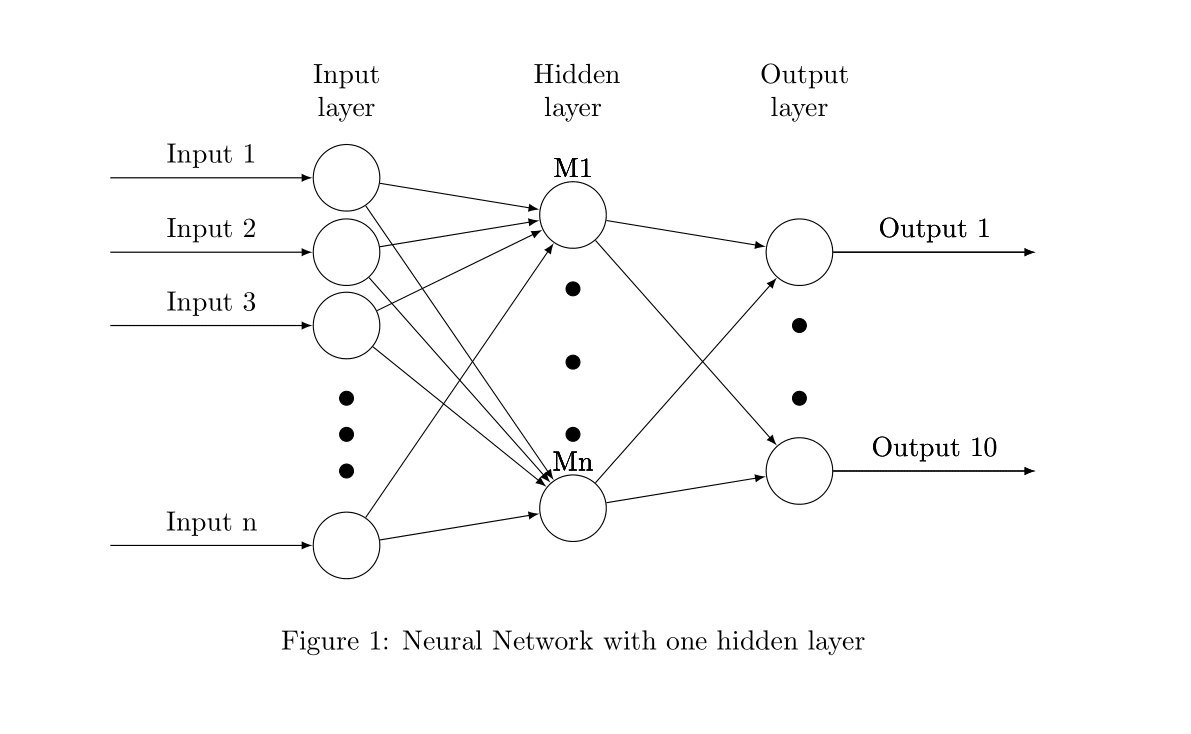
\includegraphics[width=1.10\textwidth]{../nn.png}
	\end{figure}
\newpage
\section{Feed Forward - Cost Function}

The cost function (logLikelihood plus reguralization term) we want to maximize for the problem of classifying N number of data in K categories/classes is:

$$
E(W) = \sum_{n=1}^N \sum_{k=1}^K t_{nk} \log s_{nk}   -  \frac{\lambda}{2} \left[ \left( \sum_{k=1}^K ||\mathbf{w_k^{(2)}}||^2 \right) + \left( \sum_{j=1}^M ||\mathbf{w_j^{(1)}}||^2 \right) \right], 
$$

\noindent where $s_{nk}$ is the softmax function defined as:

$$\mathbf s_{nk} = \frac{\mathbf{e^{y_{nk}}}}{\sum_{j=1}^K \mathbf{e^{y_{nk}}}},$$

\noindent where $ y_{nk}$ is the linear combination of the parameters in the hidden layer defined as:


 $$\mathbf y_{nk} = \mathbf{z}_n \mathbf{({w}_k^{(2)})}^T $$



\noindent where $z_{n}$ is the output of the selected activation function in the input layer defined as:

$$\mathbf z_{n}{(a)}, \hspace{3mm}  a = \mathbf x_{n} {(\mathbf{w_{j}}^{(1)})}^T,$$



\noindent $ \mathbf{W^{(2)}}$ is a $K \times (M+1)$ matrix, where each line represents the vector $\mathbf{{w}_k}^{(2)}$, 

\noindent $\mathbf {W^{(1)}}$ is a $(M+1) \times (D+1)$ matrix, where each line represents the vector $\mathbf{{w}_j}^{(1)}$.

\hfill



\noindent The cost function can be simplified in the following form:



$$
E(W) = \sum_{n=1}^N \left[ \left( \sum_{k=1}^K t_{nk} {(\mathbf{z}_n \mathbf{({w}_k^{(2)})}^T)} \right) - \log \left( \sum_{j=1}^K e^{\mathbf{z}_n \mathbf{({w}_j^{(2)})}^T} \right) \right]   -  \frac{\lambda}{2} \left[ \left( \sum_{k=1}^K ||\mathbf{w_k^{(2)}}||^2 \right) + \left( \sum_{j=1}^M ||\mathbf{w_j^{(1)}}||^2 \right) \right], 
$$
\newline

\noindent In the above formula we have used the fact that $\sum_{k=1}^K t_{nk} = 1$. 


\noindent We use the logsumexp trick, where m is the maximum element:
\begin{align} 
\log \sum_{j=1}^{K} e^{\mathbf{w}_j^T \mathbf{z}_n} &= \log \Bigr( \sum_{j=1}^{K} e^{\mathbf{w}_j^T \mathbf{z}_n +m -m}\Bigl) \\ 
&= \log \Bigr( \sum_{j=1}^{K} e^m e^{\mathbf{w}_j^T \mathbf{z}_n-m}  \Bigl) \\ 
&= \log \Bigr( e^m \sum_{j=1}^{K} e^{\mathbf{w}_j^T \mathbf{z}_n-m}  \Bigl) \\ 
&= \log \ e^m + \log \Bigr( \sum_{j=1}^{K} e^{\mathbf{w}_j^T \mathbf{z}_n-m}  \Bigl) \\ 
&= m + \log \Bigr( \sum_{j=1}^{K} e^{\mathbf{w}_j^T \mathbf{z}_n-m}  \Bigl) 
\end{align}

\section{Partial Derivatives of $\mathbf{w^{(1)}}$ \& $\mathbf{w^{(2)}}$ Values}
The $\mathbf{w^{(2)}}$ and $\mathbf{w^{(1)}}$ values arise from the following variables of the Cost Function: \\

\noindent $\mathbf{w^{(2)}} : \hspace{2mm} s_{nk}  \Longrightarrow  {y}_{nk} \Longrightarrow {w}_k^{(2)}$ and the Regularization Term \& \\
$\mathbf{w^{(1)}} : \hspace{2mm} s_{nk} \Longrightarrow y_{nk} \Longrightarrow z_{n} \Longrightarrow a \Longrightarrow{w}_j^{(1)}$ and the correspoding Regularization Term \\

\noindent \textbf {So, the partial derrivatives of the values $\mathbf{W^{(2)}}$ of the Cost Function are given by the following equation:}

\begin{equation} \frac{\partial E}{\partial{W^{(2)}}} = \frac{\partial E}{\partial S} \hspace{3mm}  \frac{\partial S}{\partial Y} \hspace{3mm} \frac{\partial Y}{\partial W^{(2)}}, \end{equation}

\noindent where \begin{equation} \frac{\partial E}{\partial Y}  = (T - S)^T, \hspace{2mm} \text{a }\hspace{1mm}K \times N\text{ matrix } \end{equation} 
\begin{center} {\&} 
\begin{equation} \frac{\partial Y}{\partial W^{(2)}} = Z, \hspace{2mm}\text{a }\hspace{1mm} N \times (M+1)\text{ matrix} \end{equation} \end{center}

\noindent $ \hookrightarrow $ \textbf{So, the final result for $\mathbf{W^{(2)}}$ is a
$ \textbf{K} \times \textbf{(M+1)}$ matrix as follows:}

$$ 
\textbf{(T - S)}^\textbf{Τ} \times \textbf{Z}
$$

\noindent where $T$ is a $N \times K$ matrix with the truth values of the training data, such that $[T]_{nk} = t_{nk}$, $S$ is the corresponding $N \times K$ matrix that holds the softmax probabilities and $Z$ is the $N \times (M + 1)$ matrix that holds the output of the activation function in the input layer.
\newpage

\noindent \textbf{As for $W^{\textbf{(1)}}$, the partial derrivatives of these values are given by the following equation:} \\

\begin{equation} \frac{\partial E}{\partial W^{(1)}} = \frac{\partial E}{\partial S} \hspace{3mm}  \frac{\partial S}{\partial Y} \hspace{3mm} \frac{\partial Y}{\partial Z} * \frac{\partial Z}{\partial A} \hspace{3mm}  \frac{\partial A}{\partial W^{(1)}},   \end{equation} \\

\noindent where \begin{equation} \frac{\partial E}{\partial Y}  = (T - S), \hspace{2mm} \text{a }\hspace{1mm}N \times K\hspace{1mm}\text{matrix}\text{,}\end{equation}

\begin{equation} \frac{\partial Y}{\partial Z} = W^{(2)}, \hspace{2mm}\text{a }\hspace{1mm} K \times 
(M+1)\hspace{1mm}\text{ matrix}\text{,} \end{equation} 

\begin{equation} \frac{\partial Z}{\partial A} = Z'(A),\hspace{2mm}\text{ a}\hspace{1mm} N\times (M+1)\hspace{1mm}\text{ matrix}\text{,} \end{equation}

\begin{equation} \frac{\partial A}{\partial W^{(1)}} = X, \hspace{2mm}\text{a }\hspace{1mm} N \times (D+1)\hspace{1mm}\text{ matrix}  \end{equation} \\

\noindent $ \hookrightarrow $  \textbf{So, the final result for} $ \textbf{W}^{\textbf{(1)}}$ \textbf{ is a}
$\textbf{(M+1)} \times \textbf{(D+1)}$ \textbf{matrix as follows:}

$$ 
\mathbf{(}\hspace{2mm}\textbf{(T - S)}\hspace{2mm} \textbf{W}^{\textbf{(2)}} * \mathbf{Z'(A)}\hspace{2mm}\textbf{)}^{T}  \hspace{2mm} \mathbf{Χ} $$ 

\noindent $(*) : element-wise\hspace{2mm} product $  \\

\noindent where $T$ is the matrix with the truth values of the training data, such that $[T]_{nk} = t_{nk}$, $S$ is the corresponding matrix that holds the softmax probabilities, $W^{(2)}$ is the matrix with the values of weights between the hidden layer and the output layer, Z'(A) is the matrix with the derivative of the selected activation function and $X$ is the matrix of the input data.
\newpage

\begin{lstlisting}[language = Python]
def cost_grad_softmax(w1, w2, batchX, activation, batchY, lamda):
    
    """ Compute the cost function and the partial derivatives of the weights.
    
    :param w1: The (M+1) x (D+1) matrix with the values of weights between the input layer and the hidden layer
    :param w2: The K x (M+1) matrix with the values of weights between the hidden layer and the output layer
    :param batchX: The Nb x (D+1) matrix with the current mini batch of data
    :param activation: The chosen activation function
    :param batchY: The Nb x K matrix with the binary labels of the data
    :param lamda: The positive regularization parameter
    
    :return:
        E(w): the cost of the current mini batch,
        grad_w1: (M+1) x (D+1) matrix with the partial derivatives of the weights w1 and
        grad_w2: K x(M+1) matrix with the partial derivatives of the weights w2
        
    """   
        
    a = batchX.dot(w1.T)

    z, grad_z = activations(activation, a)
    y = z.dot(w2.T)
    s = softmax(y)

    max_error = np.max(y, axis=1)
    
    # Compute the cost function to check convergence
    # Using the logsumexp trick for numerical stability 
    Ew = np.sum(batchY * y) - np.sum(max_error) - \
         np.sum(np.log(np.sum(np.exp(y - np.array([max_error, ] * y.shape[1]).T), 1))) - \
         (0.5 * lamda) * (np.sum(np.square(w1)) + np.sum(np.square(w2)))

    # Calculate gradient for w2
    grad_w2 = (batchY - s).T.dot(z) - lamda * w2
    # Calculate gradient for w1
    grad_a  = (batchY - s).dot(w2)
    grad_w1 = np.multiply(grad_a, grad_z).T.dot(batchX) - lamda * w1
    
    return Ew, grad_w1, grad_w2
\end{lstlisting}

\newpage

\section{Generate batches}
In case of Big Data we can apply \textbf{*Stohastic Gradient Ascent*} i.e. we assume that data are coming in small batches each time, instead of one sample and we make an update of the parameters by using a mini-batch of the data set. The below function generates a mini-batch every time it is called. \\

\begin{lstlisting}[language = Python]
def next_batch(X, y, batchSize):
    
    """ Generate mini batches of the training examples.
    
    :param X: The N x (D+1) input matrix with the training examples
    :param y: The N x K matrix with binary labels of the examples in X indicating the 10 categories
    :param batchSize: The chosen size of the batches
    :return: 
        X: the produced batch containing some of the examples of X
        y: the respectively labels of the examples in the batch
        
    """
    
    # Loop over our data set 'X' in mini-batches of size 'batchSize'
    for i in np.arange(0, X.shape[0], batchSize):
        # Yield a tuple of the current batched data and labels
        yield (X[i:i + batchSize], y[i:i + batchSize])
\end{lstlisting}
\newpage

\section{Runner Method - Back Propagation}

The below function runs the whole procedure. At each iteration it generates stohastic mini batches, that are fed to the algorithm in the above function \textbf{*cost\_grad\_softmax()*}. Through the training of a mini-batch, we calculate the cost of our predictions and the partial derivatives of the weights. Then, we update the weights using the derivatives and continue to the next mini-batch of the same iteration. When all mini-batches are trained in one iteration, we keep the last cost and move on to the next iteration using different mini-batches (randomly chosen). \\

\begin{lstlisting}[language = Python]
def ml_softmax_train(t, X, lamda, w1_init, w2_init, options, activation):
        
    """ Back Propagation: Call cost_grad_softmax function and updade the values of weights. 
    
    :param t: The N x K matrix with binary labels of the examples in X indicating the 10 categories
    :param X: The N x (D+1) input data matrix with ones already added in the first column
    :param lamda: The positive regularizarion parameter
    :param w1_init: The (M+1) x (D+1) matrix with the initial values of the parameters w1
    :param w2_init: The K x (M+1) matrix with the initial values of the parameters w2
    :param options: options(1) is the maximum number of iterations
                    options(2) is the tolerance
                    options(3) is the learning rate eta
                    options(4) is the size of batches
    :param activation: The chosen activation function
    :return:
        w1: the trained (M+1) x (D+1) matrix of the parameters w1
        w2: the trained K x (M+1) matrix of the parameters w2 
        costs: a list containing all the results by cost function 
        
    """

    # Generate the initial weights w1 & w2 randomly using Xavier initialization method
    w1 = np.random.rand(*w1_init.shape) * np.sqrt(1/w1_init.shape[1])
    w2 = np.random.rand(*w2_init.shape) * np.sqrt(1/w2_init.shape[1])

    # Maximum number of iteration of gradient ascend
    _iter = options[0]

    # Tolerance
    tol = options[1]


    # Learning rate
    eta = options[2]
    # Size of batches
    batchSize = options[3]

    Ewold = -np.inf
    costs = []
    
    for i in range(1, _iter+1 ):
        
        # Shuffle randomly the training examples and respectively their labels on each iteration,
        # in order to implement stohastic gradient ascent
        permutation = np.random.permutation(len(X))
        X = X[permutation,:]
        t = t[permutation,:]
        
        # Generate mini-batches after shuffling the data set
        for (batchX, batchY) in next_batch(X, t, batchSize):
        
            # Calculate cost and partial derivatives of the parameters w1 & w2 for each mini-batch and iteration
            Ew, grad_w1, grad_w2 = cost_grad_softmax(w1, w2, batchX, activation, batchY, lamda)
            
            # Update parameters based on gradient ascent
            w1 = w1 + eta * grad_w1
            w2 = w2 + eta * grad_w2
            
        # Save cost produced by the last mini batch
        costs.append(Ew)
        
        # Show the current cost function on screen
        if i % 50 == 0:
            print('Iteration : %d, Cost function :%f ' % (i, Ew))

        # Break if you achieve the desired accuracy in the cost function
        if np.abs(Ew - Ewold) < tol:
            break
                

        Ewold = Ew

    return w1, w2, costs
\end{lstlisting}

\newpage 
\section{Select Activation Function}

Through the three options described above (logarithm, tangent, cosine), user has to select the desired one from the standard input. \\

\begin{lstlisting}[language = Python]
def selectActivation(): 
    
    """ Selects the number from standard input, which indicates the desired activation function. 
    
    :return: The selected activation function
    
    """
    
    # While you do not select an integer between 1-3 continue
    while True:
        try:
            # Read integer from stdin
            act = int(input("Select 1 of the following numbers based on the desired Activation Function:\n \
                            \n 1: logarithm function \n 2: tangent function \n 3: cosine function\n"))
            print("")
            if(act in range(1,4)):
                break;
            else:
                raise ValueError('Invalid input. Please select again an integer between 1-3!')
        except ValueError:
            print("")
            print("Invalid input. Please select again an integer between 1-3!")
            print("")
            
    # Case1: input = 1
    if(act == 1):
        activation = "log"
        print("You selected Logarithm Activation Function!")
    # Case2: input = 2
    elif (act == 2):
        activation = "tan"
        print("You selected Tangent Activation Function!")
    # Case3: input = 3
    elif(act == 3):
        activation = "cos"
        print("You selected Cosine Activation Function!")
        
    return activation
\end{lstlisting}

\newpage

\section{Gradcheck}

When implementing gradient-based methods, it is suggested to include numerical gradient check (gradcheck). \\

\noindent Numerical approximation of the partial derivatives of $W^{(1)}$ \& $W^{(2)}$ : \\


\begin{equation} \frac{\partial E}{\partial W^{(1)}} \approx \frac{E{(W^{(1)} + ε)} - E{(W^{(1)} - ε)}}{2ε} \end{equation}

\begin{equation} \frac{\partial E}{\partial W^{(2)}} \approx \frac{E{(W^{(2)} + ε)} - E{(W^{(2)} - ε)}}{2ε} \end{equation}

${( ε = 10^{-6})} $

\begin{lstlisting}[language = Python]
def gradcheck_softmax(w1_init, w2_init, X, t, lamda, activation):
    
    """ Check if the equations of the partial derivatives are correct.
    
    :param w1_init: The (M+1) x (D+1) matrix with the initial values of the parameters w1
    :param w2_init: The K x (M+1) matrix with the initial values of the parameters w2
    :param X: The N x (D+1) input data matrix with ones already added in the first column
    :param t: The N x K matrix with binary labels of the examples in X indicating the 10 categories
    :param lamda: The positive regularization parameter
    :param activation: The chosen activation function
    :return:
        grad_w1: The computed partial derivatives of the weights w1
        numericalGrad1: The approximate values of the derivatives of the weights w1
        grad_w2: The computed partial derivatives of the weights w2
        numericalGrad2: The approximate values of the derivatives of the weights w2
        
    """
    
    # Generate the initial weights w1 & w2 randomly using Xavier initialization method
    w1 = np.random.rand(*w1_init.shape) * np.sqrt(1/w1_init.shape[1])
    w2 = np.random.rand(*w2_init.shape) * np.sqrt(1/w2_init.shape[1])
    
    epsilon = 1e-6

    _list = np.random.randint(X.shape[0], size=5)
    x_sample = np.array(X[_list, :])
    t_sample = np.array(t[_list, :])
    
    Ew, grad_w1, grad_w2 = cost_grad_softmax(w1, w2, x_sample, activation, t_sample, lamda)
    
    numericalGrad1 = np.zeros(grad_w1.shape)
    numericalGrad2 = np.zeros(grad_w2.shape)
    
    # Compute all numerical gradient estimates for w1 and store them in
    # the matrix numericalGrad1
    for k in range(numericalGrad1.shape[0]):
        for d in range(numericalGrad1.shape[1]):
            
            # Add epsilon to the w[k,d]
            w_tmp1 = np.copy(w1)
            w_tmp1[k, d] += epsilon
            e_plus1, _ , _= cost_grad_softmax(w_tmp1, w2,  x_sample, activation, t_sample, lamda)
            
            # Subtract epsilon to the w[k,d]
            w_tmp1 = np.copy(w1)
            w_tmp1[k, d] -= epsilon
            e_minus1, _ , _ = cost_grad_softmax(w_tmp1, w2, x_sample, activation, t_sample, lamda)
            
            # Approximate gradient ( E[ w[k,d] + theta ] - E[ w[k,d] - theta ] ) / 2*e
            numericalGrad1[k, d] = (e_plus1 - e_minus1) / (2 * epsilon)
    
    # Compute all numerical gradient estimates for w2 and store them in
    # the matrix numericalGrad2
    for m in range(numericalGrad2.shape[0]):
        for n in range(numericalGrad2.shape[1]):
            
            # Add epsilon to the w[k,d]
            w_tmp = np.copy(w2)
            w_tmp[m, n] += epsilon
            e_plus2, _ , _ = cost_grad_softmax(w1, w_tmp, x_sample, activation, t_sample, lamda)

            # Subtract epsilon to the w[k,d]
            w_tmp = np.copy(w2)
            w_tmp[m, n] -= epsilon
            e_minus2, _ , _ = cost_grad_softmax(w1, w_tmp, x_sample, activation, t_sample, lamda)
            
            # Approximate gradient ( E[ w[k,d] + theta ] - E[ w[k,d] - theta ] ) / 2*e
            numericalGrad2[m, n] = (e_plus2 - e_minus2) / (2 * epsilon)
    return (grad_w1, numericalGrad1, grad_w2, numericalGrad2)
\end{lstlisting}
\newpage

\section{Run Gradcheck Function}
The below function runs the Gradcheck function and finds the estimated difference between the computed partial derivatives and the approximate ones. We expect insignificant difference between them, in order to ensure about the correctness of our computations, otherwise there is an error in the equations of the derivatives. \\


\begin{lstlisting}[language = Python]
# N: number of training data
# D: number of feautures, plus the one of bias
N, D = X_train.shape

# Number of categories
K = 10 
# Number of hidden units
M = 100 

# Initialize w1 & w2 weights for gradient ascent, such it has same number of columns as our input features
w1_init = np.zeros((M, D))
w2_init = np.zeros((K, M))

# Regularization parameter
lamda = 0.1

# Activation function
activation = selectActivation()

# Calculate the partial derivatives and the approximate derivatives of the weights w1 & w2
grad_w1, numericalGrad1, grad_w2, numericalGrad2 = gradcheck_softmax(w1_init, w2_init, X_train, y_train, lamda, activation)

# Compare partial derivatives with the approximate ones and print the estimated difference
print( "The difference estimate for gradient of w1 is : ", np.max(np.abs(grad_w1 - numericalGrad1)) )
print( "The difference estimate for gradient of w2 is : ", np.max(np.abs(grad_w2 - numericalGrad2)) )
\end{lstlisting}

\newpage

\section{Training}

\begin{lstlisting}[language = Python]
# N: number of training data
# D: number of feautures, plus the one of bias
N, D = X_train.shape

# Number of categories
K = 10
# Number of hidden units
M = 300 

# Initialize w1 & w2 weights for gradient ascent
w1_init = np.zeros((M, D))
w2_init = np.zeros((K, M))

# Regularization parameter
lamda = 0.01

# Check if activation variable is defined, otherwise select activation function
try:
    activation
except NameError:
    activation = selectActivation()

# options for gradient ascent
# i.e. maximum number of iterations, tolerance, learning rate, size of batches
options = [300, 1e-6, 0.001, 256]

# Train the model
w1, w2, costs = ml_softmax_train(y_train, X_train, lamda, w1_init, w2_init, options, activation)
\end{lstlisting}

\newpage

\section{Plot Cost Function}

\begin{lstlisting}[language = Python]
# Plot cost versus number of iterations
plt.plot(np.squeeze(costs))
plt.ylabel('cost')
plt.xlabel('iterations (per tens)')
plt.title("Learning rate =" + str(format(options[2], 'f')))
plt.show()
\end{lstlisting}

\hfill

\section{Testing}
After training our model, we have to test it using the test data set without the labels. \\

\begin{lstlisting}[language = Python]
def ml_softmax_test(w1, w2, X_test, activation):
    
    """ Finds the category in which each example belong to.
    
    :param w1: The trained (M+1) x (D+1) matrix of the parameters w1
    :param w2: The trained K x (M+1) matrix of the parameters w2
    :param X_test: The matrix with the data that will be used for testing
    :param activation: The chosen activation function
    :return:
        ttest: The (N x 1) matrix that contains the predict category of each example
    
    """
    
    a = X_test.dot(w1.T)
    z, grad_z = activations(activation, a)
    y = z.dot(w2.T)
    ytest = softmax(y)
    # Keep the position with the biggest probability, as the category a test example belongs to
    ttest = np.argmax(ytest, 1)
    
    return ttest
\end{lstlisting}


\subsection{Call Test Function for Train Data Set}

\begin{lstlisting}[language = Python]
pred = ml_softmax_test(w1, w2, X_train, activation)
\end{lstlisting}


\noindent \textbf{Train Accuracy}
\begin{lstlisting}[language = Python]
# Compare our predictions with the real values and compute the train accuracy of the model
np.mean( pred == np.argmax(y_train,1) )
\end{lstlisting}
\newpage

\subsection{Call Test Function for Test Data Set}

\begin{lstlisting}[language = Python]
pred = ml_softmax_test(w1, w2, X_test, activation)
\end{lstlisting} 
\hfill

\noindent \textbf{Test Accuracy}
\begin{lstlisting}[language = Python]
# Compare our predictions with the real values and compute the test accuracy of the model
np.mean( pred == np.argmax(y_test,1) )
\end{lstlisting}

\hfill
\newline

\section{Misclassified Test Data}

\subsection{Plot Mnist's Faults}
\begin{lstlisting}[language = Python]
def plot_mnists_faults():
    
    """ Plot 25 random misclassified images from the Mnist training set. """  

    
    faults = np.where(np.not_equal(np.argmax(y_test,1),pred))[0]

    # plot 25 misclassified examples from the test set
    n = 25
    samples = np.random.choice(faults, n)
    sqrt_n = int( n ** 0.5 )

    plt.figure( figsize=(11,13) )

    cnt = 0
    for i in samples:
        cnt += 1
        plt.subplot( sqrt_n, sqrt_n, cnt )
        plt.subplot( sqrt_n, sqrt_n, cnt ).axis('off')
        plt.imshow( X_test[i,1:].reshape(28,28)*255, cmap='gray' )
        plt.title("True: "+str(np.argmax(y_test,1)[i])+ "\n Predicted: "+ str(pred[i]))

    plt.show()
\end{lstlisting}
\newpage

\subsection{Plot Cifar-10 Faults}
\begin{lstlisting}[language = Python]
def plot_cifar_faults():
    
    """ Plot 25 random misclassified images from the Cifar-10 training set. """  
    
    faults = np.where(np.not_equal(np.argmax(y_test,1),pred))[0]

    n = 25
    sqrt_n = int( n**0.5 )
    samples = np.random.choice(faults, n)

    plt.figure( figsize=(15,15) )

    cnt = 0
    for i in samples:
        arr = X_test[i, 1:] * 255
        R = arr[0:1024].reshape(32,32)/255.0
        G = arr[1024:2048].reshape(32,32)/255.0
        B = arr[2048:].reshape(32,32)/255.0

        img = np.dstack((R,G,B))
        cnt += 1
        plt.subplot( sqrt_n, sqrt_n, cnt )
        plt.subplot( sqrt_n, sqrt_n, cnt ).axis('off')
        plt.imshow(img,interpolation='bicubic')
        plt.title("True: "+str(np.argmax(y_test,1)[i])+ "\n Predicted: "+ str(pred[i]))

    plt.show()
\end{lstlisting}
\hfill
\hfill
\subsection{View Misclassified Data}

\begin{lstlisting}[language = Python]
if(data_set == 1):
    plot_mnists_faults()
elif(data_set == 2):
    plot_cifar_faults()
\end{lstlisting}

\nocite{*}
\bibliography{jupyter} 
\underline{}
\bibliographystyle{ieeetr}
\end{document}
